\section{Critical explorations and oriented loops}
\label{sec:critical}

The scalar limit established in Proposition~\ref{prop:quenched-cardy}
does not determine the joint law of crossings.  Our first step towards
that law is to identify the critical interfaces, while keeping the
tessellation fixed.  The argument has three stages.  First we identify
the law of an exploration stopped on a crosscut, including its unexplored
domain.  We then recover the ordered path from these stopped domains.
Finally we explore inside the remaining faces to obtain the oriented
interface loops.  Section~\ref{sec:critical-tests} will read the crossing
tests needed for the near-critical argument from this common loop law.

Throughout this section we work along a deterministic sequence of
tessellations supplied by Lemma~\ref{lem:good-sequences}.  Thus mesh
sizes on compact sets tend to zero, fixed polygon crossing probabilities
converge to Cardy's formula, and the fixed-scale conclusions of
Lemmas~\ref{lem:color-arms} and~\ref{lem:boundary-arms} hold.  All
probabilities in the section concern independent fair colors on these
fixed tessellations.  When boundary values are prescribed, only the
interior colors are random.  Every arm estimate is used with the mesh
limit first and the radii fixed; subsequently the inner radius may
decrease.  In particular, no estimate conditioned on an arbitrary
already explored color configuration is being asserted.

\subsection{Exploration on a fixed triangulation}

We use the embedded triangulation of sites described in
Section~\ref{sec:inputs}.  A graph disk is the closed region inside a
simple site cycle, together with the triangles it contains.  We choose
the cycle without chords in its interior.  Two specified boundary edges
are switches: the boundary sites between them on one arc are black, and
those on the other arc are white.  The interface is drawn through each
triangle between its black and white corners.  It starts at one switch
and ends at the other.  At each step it queries an as yet unknown site
only if that site's color is needed to choose the next edge.  Equivalent
drawings on Voronoi edges differ by a quantity tending to zero with the
mesh.

Curves are considered modulo increasing reparametrization, with the
uniform distance between representatives; constant pauses are
irrelevant.  Boundary convergence in order means convergence in this
curve metric with the cyclic orientation retained.  A sequence of graph
disks approximates a Jordan domain if its boundary cycles converge in
order to the Jordan boundary and its marked switch edges converge to the
specified distinct marks.

\begin{proposition}[Chordal exploration convergence]
\label{prop:chordal}
Let graph disks on a deterministic sequence as above approximate a
bounded Jordan domain $D$, with switches converging to distinct boundary
points $a,b$.  Give their interiors independent fair colors and their
two boundary arcs the prescribed opposite colors.  The exploration from
$a$ to $b$ converges in law, in the curve metric, to chordal
$\mathrm{SLE}_6$ in $D$ from $a$ to $b$.  This conclusion holds for every
such converging sequence of disks and marks.
\end{proposition}

We prove the proposition in the present and next two subsections.  The hull
identification follows the method of Camia and Newman
\cite{cnexploration}; the graph, boundary, and conditional-law arguments
below establish its applicability here.  The convergence theorem in
\cite{cnexploration} is not used as a theorem about the present
triangulations.

The first observation explains why exploration can be continued without
resampling the geometry or changing the conditional color law.  Include
the original boundary cycle, every vertex in the band of triangles
visited by the exploration, and every edge between included vertices in
the revealed graph.  Unqueried sites outside this graph retain their
independent fair colors, conditional on the exploration.  Indeed an
exploration history specifies only the queried colors; the decision to
query a site is a function of the preceding answers and the fixed
triangulation.  Summing over histories with the same revealed data does
not impose any additional constraint on unqueried coordinates.

\begin{lemma}[Faces of the revealed band]
\label{lem:revealed-faces}
The revealed graph is two-connected.  Each of its faces that contains
unqueried sites has a simple, internally chord-free site cycle as
boundary.  For a nonempty explored band, such a cycle shares at most one interval
with the original boundary cycle; the interval may be empty or a single
vertex.  After a
completed exploration every such face has a monochromatic boundary.
If an exploration is stopped with its outgoing edge facing the
unqueried face containing the target switch, that face has exactly two
switches, namely the target and the outgoing edge.
\end{lemma}

\begin{proof}
Begin with the boundary cycle.  Adding the successive triangles of the
exploration band preserves two-connectivity: a triangle is attached
along the edge through which it is entered, and any new corner has two
neighbors in the graph already present.  Adding the remaining edges
between revealed vertices preserves this property.  Boundaries of
bounded faces of a two-connected plane graph are simple cycles.  An
interior chord would be an edge between revealed vertices and would
already have split the face, proving the chord assertion.

The part of the visited band off the original boundary is connected.
Two successive steps have an interior corner in common whenever they
meet the boundary: otherwise the common edge would be an interior chord
of the initial cycle.  The initial and final switch triangles cause no
exception to this connectivity.  If a face had two separate intervals
on the original boundary, a crosscut through that face between two of
its boundary contacts would leave parts of this connected interior band
on both sides.  They could not be joined without crossing the crosscut
or the face.  This proves the interval assertion, including an isolated
contact vertex by taking a small crosscut around that vertex.

Draw the exploration as a simple dividing arc in the triangulated disk.
Its black neighbors are on one bank and its white neighbors on the
other; an edge joining the two banks belongs to the visited band.
Consequently a complementary face sees only one color on its boundary.
For the target face at a stop, continue the dividing arc through that
face to the target.  The same separation gives one black and one white
boundary arc, meeting at the stated edges.
\end{proof}

We next establish the compactness and contact properties needed both
for stopped explorations and for recursion in the faces.  Work first in
round disk coordinates.  For initial Jordan approximations their
conformal maps converge uniformly on the closed disk.  The coordinate
mesh tends to zero by Lemma~\ref{lem:chart-cardy}: a sequence of
connected triangles with physical diameter tending to zero and
coordinate diameter bounded below would yield a nondegenerate
continuum on which the limiting map is constant.  The same observation
will apply to the maps of residual domains once their uniform
convergence has been proved.

\begin{lemma}[Tightness of paths and face boundaries]
\label{lem:exploration-tightness}
Exploration paths are tight in the curve metric.  The same holds jointly
for boundaries of faces produced by a completed exploration and for
the two colored arcs of a stopped target face.  At any fixed positive
scale their numbers of annular traversals are tight.  These statements
hold in the disk coordinates just described and, by uniform continuity
of the conformal maps, in physical coordinates.
\end{lemma}

\begin{proof}
We use the multiple-crossing compactness argument of
Aizenman and Burchard~\cite{aizenmanburchard99}, spelling out its
fixed-scale application to these paths and face boundaries.
Cut a wall traversal between two graph cycles in a buffered annulus.
Following the corners of the successive triangles on either bank gives
a connected site path, its \emph{shadow}.  Crop the shadow farther from
the two ends so that it cannot run around an end of the wall traversal.
Between disjoint proper wall traversals the corresponding shadows lie
in the intervening gaps.  Thus many traversals supply many site-disjoint
arms, with at most a fixed loss at the ends.  A positive fraction of
these arms have one color.  The BK inequality
\cite[Theorem~3.3]{vandenbergkesten85}, together with the
positive probability of an opposite-color circuit in a fixed-ratio
subannulus, bounds the probability of arbitrarily many such arms by a
geometric tail.  Increasing the annulus ratio if necessary makes the
one-crossing bound strictly less than one.

In a boundary half-annulus, $k$ disjoint proper wall traversals have at
least $k-1$ free shadows, in their internal gaps.  Here and below
\emph{free} means that the arm uses only random interior sites.  The
original boundary sites can occur only in the two outside gaps.  If
neither bank of any traversal uses those sites, the two outside shadows
are free as well, giving $k+1$ free arms.  These assertions can be read
between intermediate graph crosscuts and then cropped, so that a large
site star cannot join around a cut.  They depend only on the plane
triangulation.  Lemma~\ref{lem:boundary-arms} and the same BK argument
give the boundary estimates.  For a face boundary the random pieces
are monochromatic simple site paths.  Its original-boundary pieces and
switches are bounded in number and cause no additional oscillations.
The free pieces obey the preceding arm bounds.  Near each fixed switch
use the fixed-point one-arm bound instead.

For clarity, fixed-annulus estimates suffice for tightness in the
curve metric.  Fix an excursion size $r>0$.  Cover first the switches,
then the boundary, and then the remaining compact interior by finitely
many smaller neighborhoods whose surrounding annuli have outer
diameter less than $r/10$.  Every successive displacement of size $r$
requires a traversal of one of these annuli.  Their crossing counts
therefore bound the number of such displacements.  Do this for
$r=2^{-j}$.  Choose bounds with exceptional probabilities summable in
$j$, and parametrize curves by assigning summably small time budgets
to their successive steps at each scale.  This gives a common modulus
of continuity outside an arbitrarily small exceptional event.  The
same bounds apply simultaneously to face boundaries, since their
crossings are among the site arms just counted.  Finite initial mesh
indices can be accommodated separately.  The nondegeneration argument
in Lemma~\ref{lem:face-convergence} below supplies the finite numbers of
macroscopic faces needed to list those boundaries jointly.
\end{proof}

\begin{lemma}[Contact rules]
\label{lem:exploration-contacts}
In a subsequential curve limit, the exploration has no interior triple
point, no double point on the original boundary, and no second visit
to either switch.  Its interior double points avoid every fixed line
segment.  It has no nonconstant interval lying on the boundary.
Moreover a discrete excursion whose bank shadows avoid a specified
boundary bank cannot acquire an intermediate contact with that bank
in the limit, provided the positions immediately before and after that
contact make positive excursions from it.

For a random monochromatic arc of a face boundary, distinct interior
visits to the same point are excluded.  On an original boundary
interval of its own color it cannot have an intermediate contact
between positive excursions.  A face of positive limiting diameter
cannot attach to a boundary interval of its own color through an
interval collapsing to a point, including a single-vertex attachment.
These statements also hold with the colors reversed.
\end{lemma}

\begin{proof}
We first identify the arms forced by a contact.  All traversals below
are properly trimmed in a buffered annulus, so that their shadows
cannot join around an annular end.

\emph{Exploration contacts.}
A triple visit in the bulk, with positive excursions between visits,
gives six wall traversals and hence six free arms.  A double visit
on the original boundary gives four traversals and three free arms.
A double visit on a fixed interior segment gives four free arms.
If a wall comes to a boundary bank and leaves it without either
shadow using that bank, the two traversals have three free shadows.
A shadow uses a bank site only when a crossed edge is incident with
that site, up to one triangle, so this count is independent of the
precise wall drawing.  A second visit to a specified switch requires
a free arm from a vanishing neighborhood of that point.  A
nonconstant interval of the wall on the boundary likewise gives
such an arm at some point of a fixed countable dense set of boundary
points.

\emph{The exterior of a face.}
A monochromatic face arc needs an additional planar observation.
At a finite mesh let $C$ be the simple site cycle bounding the face.
Every site on its random part has an opposite-colored neighbor
across an edge of the explored band.  These neighbors belong to one
connected opposite-colored bank, denoted by $K$, which includes its
original boundary arc and lies in the closed exterior of $C$.
Suppose four properly trimmed traversals of the random part of $C$
cross a bulk annulus.  Each traversal has an exterior-side
incidence with a neighboring gap, and one gap accounts for at most two of these incidences.
Thus at least two distinct gaps abut a traversal on its exterior
side.  Other pieces of $C$ may still enter such a gap.  We show
that each selected gap contains an opposite-colored radial crossing.

Choose one of these gaps between two proper traversals $P,Q$ of
a wider annulus, with the gap on the exterior side of $P$.  Cut
across this gap at two intermediate graph
curves, leaving the ends of $P,Q$ beyond the cuts.  The resulting
working quadrilateral has subarcs of $P,Q$ as its lateral sides,
and its interior avoids the whole of $P$ and $Q$; this construction
allows radial backtracks.  Write $p_-,p_+$ for the ends of the
contiguous face-cycle subarc $P$, and join their opposite neighbors
to them by short spokes beyond the working cuts.  If $K$ has no
longitudinal crossing of the quadrilateral, rectangle separation
supplies a transverse crosscut avoiding $K$, from an interior point
$x$ of $P$ to $Q$, with interior disjoint from all of $P$.
Stop it at its first subsequent meeting $y$ with the entire cycle
$C$.  It starts on the exterior side of $P$, so this prefix lies
in the exterior.  Other pieces of $C$ may cause an earlier stop,
but $y$ is outside $P$ because the original crosscut avoids $P$.

The relevant ambient region is the whole exterior of $C$,
compactified by the point at infinity: it is a topological disk.
The boundary points occur in the cyclic order $p_-,x,p_+,y$.
Our crosscut therefore separates the two endpoint spokes in this
disk.  The spokes avoid its working annulus and put their
opposite-colored endpoints in different components.  Those
endpoints cannot be joined by $K$ without crossing the crosscut,
a contradiction.  In particular a connection going around an end
of the annulus does not escape this separation.  Crop once more
to remove the short spokes.  The resulting opposite-colored
crossings in the two selected gaps are disjoint; with the
four monochromatic traversals they supply six free arms.

A self-return of the random face arc in the bulk forces exactly
this configuration.  Near the original boundary, four free
traversals already exceed the three-arm requirement.  If the face
arc has the same color as the nearby original bank, an intermediate
contact gives two arms along the arc and one opposite arm from $K$.
The opposite arm cannot use that original bank, so all three arms
are free.  The same count applies when the two ends of a macroscopic
face arc approach each other as its shared boundary interval
collapses; a singleton attachment is included.  At a fixed switch
or fixed patch endpoint, one free arm suffices.  Contacts with an
original bank of the other color need not be excluded: they will
be retained as distinct boundary accesses.

\emph{Applying the arm estimates.}
For a fixed positive outer excursion scale, cover the compact
interior by $O(r^{-2})$ balls of radius $r$.  The six-arm bound in
Lemma~\ref{lem:color-arms}, whose exponent is greater than two,
excludes both interior triple visits of the wall and self-returns
of a face arc.  Along a boundary interval there are only
$O(r^{-1})$ balls, and the free three-arm exponent $4/3>1$ in
Lemma~\ref{lem:boundary-arms} excludes the boundary configurations
just listed.  The four-arm exponent greater than one similarly
excludes double visits on a fixed interior segment.  The fixed-point
one-arm estimate handles switches, patch endpoints, and the dense
boundary tests.

All centers and outer radii are fixed before passing to the mesh
limit.  A contact at a random point with positive excursions is
covered by an enlarged ball of a rational grid.  Exhaust excursion
sizes by a countable list and then decrease the grid scale.  Thus
none of these exclusions requires an arm estimate conditioned at a
random limiting contact point.
\end{proof}

\begin{lemma}[Convergence of the remaining faces]
\label{lem:face-convergence}
After a completed exploration, every nonconstant subsequential limit
of a remaining face boundary is a Jordan curve.  Its interior is a
component of the complement of the limiting exploration in the
initial domain.  Faces of diameter at least any fixed $r>0$ have tight
numbers, converge without surplus faces, and retain their colors and
their intervals of attachment to the original boundary.  Thresholds
on diameters may be chosen outside the atoms of the limiting sizes.
\end{lemma}

\begin{proof}
A face boundary consists of its random part and at most one interval
of the initial boundary, by Lemma~\ref{lem:revealed-faces}.  The random
part has no self-return, by Lemma~\ref{lem:exploration-contacts}.  If
there is an original boundary interval, it has the face's color.  The
same lemma excludes an intermediate return to that interval or an
additional visit to its endpoints.  A nontrivial interval cannot have
the entire free arc collapse, because its two endpoints are separated
in the initial Jordan boundary parametrization; intervals under
consideration contain no switch in their interior.  Nor can a
macroscopic free part have its attachment interval collapse.  If no
original interval is present, a nonconstant limiting cycle cannot
fold into a doubly traced arc: that would be a distinct visit of its
random part.  After deleting pauses the limit is therefore Jordan.

These facts also give the claimed finiteness.  If arbitrarily many
disjoint faces had diameter at least $r$, their inscribed radii would
have a subsequence tending to zero.  Curve tightness would give a
nonconstant limiting boundary of such a subsequence.  Its Jordan
interior contains a disk; convergence in order forces the
approximating face to contain a slightly smaller disk, a contradiction.
The argument proves tightness of the number and excludes surplus
macroscopic faces in any coupled subsequential limit.

The face boundaries lie within a vanishing distance of the band or
the initial boundary.  Jordan convergence prevents the band from
entering a limiting face interior.  Conversely a compact ball in an
open component off the limiting trace, together with finitely many
compact joining paths in that component, eventually avoids the
discrete band.  It is thus recovered by one of the discrete faces.
This identifies the components.  The side of a fixed point off the
trace is preserved by the winding number of the wall completed along
the initial boundary, so the color labels pass to the limit.  Finally
a nontrivial original boundary interval cannot be supplied entirely
by the limiting free arc: this would contradict the fixed-point
one-arm test on that interval.  Hence true intervals of attachment,
as well as their order, are recovered.
\end{proof}

\subsection{Stopping on a crosscut and identifying the residual domain}

Fix a smooth crosscut $L$ in the current disk coordinates, separating
the start from the target.  We call its two complementary portions the
front and the back, with the start in the front.  The cuts used for
iteration will be images of semicircles centered at $0$ in the upper
half-plane with marks $0,\infty$.  Approximate $L$ by a simple graph
crosscut whose intermediate vertices are interior.  Stop the
exploration \emph{before} it queries a vertex of that crosscut.  If it
passes the crosscut at an endpoint along boundary triangles, stop at
the first triangle in that endpoint star instead.  Such endpoint
stops will have vanishing probability when the endpoint neighborhoods
are shrunk after the mesh limit.

\begin{lemma}[The stopped target face]
\label{lem:stopped-domain}
At a stop separated from the two endpoints of $L$, the outgoing edge
faces the unqueried component containing the target.  In a coupled
subsequential limit its boundary consists of two individually simple
colored banks, joining the new tip to the target, in prime-end order.
In the current coordinates the target domain is the union of the
back, two Jordan side domains in the front, and their two open
attaching intervals on $L$.  The two colored side arcs meet $L$ only
at their prescribed endpoints, one of which is the hit point.
Normalized conformal maps onto the new target domains converge
uniformly on their closed parameter disks.  The same is true of the
composed maps into the original physical domain.
\end{lemma}

\begin{proof}
Until the stopping query, every interior vertex of the separating
path is unknown.  Its bulk portion joins, through unknown vertices
on the back side, the target edge.  The chord-free initial boundary
ensures a connected inner row at that edge: the triangles adjacent
to consecutive boundary edges meet through their interior corner
stars.  Consequently the outgoing edge is incident to the target
face.  This argument is applied outside fixed endpoint
neighborhoods; chords from the crosscut to the rim near its ends
cannot affect it.  Lemma~\ref{lem:revealed-faces} gives the two
colored boundary arcs of that face.

With probability tending to one as endpoint neighborhoods decrease,
the portions of the original banks from the target up to, and a
little beyond, the endpoints of $L$ remain untouched.  To reach one
of these fixed neighborhoods, the band's bank of the opposite color
must supply a free arm out of it.  The fixed-point one-arm bound
therefore applies.  Each target-face arc consists of an original
bank followed by random sites of the same color.  Away from the
termination, its simplicity follows from
Lemma~\ref{lem:exploration-contacts}.  There is one additional check
at the separator: an extra approach of a random arc to $L$, with
positive excursions of that arc before and after it, supplies two
arms along the arc and an opposite arm through its neighbors in the
band.  All three arms lie on the front side of $L$, up to the
vanishing mesh error.  Lemma~\ref{lem:boundary-arms}, applied in
this smooth crosscut patch, excludes such an approach.  The same
count excludes an additional visit to the termination.  The fixed
endpoint tests handle the two ends of $L$.

The residual face is now described without identifying distinct
boundary accesses.  In the discrete target face the separator goes
from one old bank to the other, and the queried vertex would be
next to the endpoints of the outgoing edge.  Cutting there, and
removing that one triangle if necessary, separates two side
polygons from the back.  In the limit each side polygon has a
boundary formed by a subinterval of its own old bank, its simple
random arc, and its subarc of $L$.  This is a Jordan curve by the
contact exclusions.  An encounter with the other-colored bank does
not create a repeated point of this side curve: that other bank is
not part of its boundary traversal.  The two side disks may touch
each other in their closed exteriors.  They remain joined to the
back through the two \emph{open} seams, not through the hit point.
Figure~\ref{fig:stopped-domain} records the order of these pieces.

This decomposition proves kernel convergence: compact subsets of
each side interior, the back, and the open seams persist; compact
joining paths in the displayed union also persist.  It specifies
the limiting prime ends.  On the interior of each piece of side
boundary one uses its Jordan access, even when another bank touches
its image.  Near an attaching endpoint one joins the Jordan
neighborhoods through the incident open seam.  At the hit point
the two neighborhoods are joined through the back.  Thus the
boundary traversal is continuous in exactly the order of the
discrete cycles.

For the required uniform convergence of maps, use the admissible
domain version of boundary convergence in
\cite[Lemma~A.1 and Corollaries~A.1--A.2]{cnexploration}.
Its hypotheses are as follows: the boundary is the ordered union
of three individually simple arcs $J_1,J_2,J_3$; $J_3$ avoids the
interiors of the other two arcs and is accessible from the
exterior at each of its points; and the three corresponding
boundary arcs converge in the uniform curve metric.  The other
two arcs are allowed to touch.  Here choose $J_3$ to be a closed
arc around the target strictly inside the untouched round part of
the boundary.  The remaining boundary, divided at the hit point,
gives $J_1,J_2$.  Their separate simplicity and their convergence
were just proved; $J_3$ has exterior accesses in the round disk
and misses their interiors.  The approximating Jordan graph disks
meet the same conditions.  A normalization point can be fixed in
the back, and the two marked version gives convergence of the
start and target prime ends.  The cited corollaries therefore give
uniform convergence of maps on the closed disk.  Composing with
the preceding uniformly convergent maps proves the physical
statement.  Equivalently, marks chosen in boundary order converge
because a sequence of boundary subarcs of diameter tending to zero
cannot have preimages of positive diameter: that would make a
nonconstant limiting parameter arc constant under the limiting
map.
\end{proof}

\begin{figure}[tb]
\centering
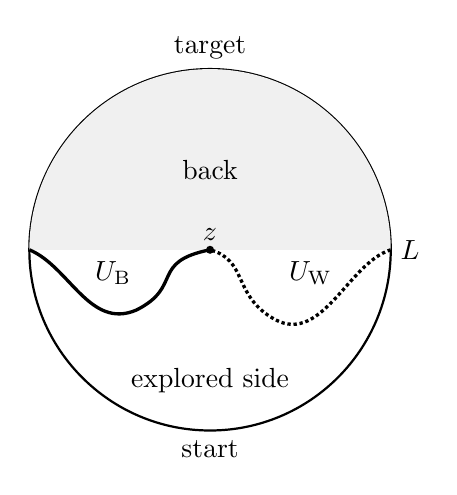
\begin{tikzpicture}[scale=0.85]
  \draw[thick] (0,0) circle (2.7);
  \draw[dashed] (-2.7,0)--(2.7,0);
  \fill[gray!12] (-2.7,0) arc[start angle=180,end angle=0,radius=2.7]
       --cycle;
  \draw[very thick] (-2.7,0) .. controls (-2.1,-.25) and (-1.8,-1.2) ..
       (-1.1,-.9) .. controls (-.4,-.55) and (-.9,-.18) .. (0,0);
  \draw[very thick,densely dotted] (2.7,0) .. controls (2.05,-.2) and
       (1.65,-1.5) .. (.9,-1) .. controls (.35,-.65) and (.55,-.15) .. (0,0);
  \fill (0,0) circle (.06);
  \node[above] at (0,0) {$z$};
  \node at (0,1.2) {back};
  \node at (-1.45,-.35) {$U_{\mathrm B}$};
  \node at (1.5,-.35) {$U_{\mathrm W}$};
  \node[below] at (0,-2.7) {start};
  \node[above] at (0,2.7) {target};
  \node[right] at (2.7,0) {$L$};
  \node at (0,-1.95) {explored side};
\end{tikzpicture}
\caption{The stopped target domain in current disk coordinates,
schematically.  The two side domains $U_{\mathrm B},U_{\mathrm W}$
attach to the back along the open parts of $L$ on either side of the
hit $z$.  Their simple colored boundary arcs may touch in physical
projection; the accesses in the displayed boundary order remain
distinct.  The picture suppresses portions already cut off by the
exploration.}
\label{fig:stopped-domain}
\end{figure}

We now identify the law of these domains.  The argument also applies
when the preceding coordinate map has a nonsimple boundary image,
provided its two banks are separately simple and its closed-disk maps
converge uniformly.  This qualification matters after the first stop.

\begin{lemma}[Cardy determines the stopped kernel]
\label{lem:stopped-kernel}
The joint limiting law of the hit on $L$ and the two side domains of
Lemma~\ref{lem:stopped-domain} is uniquely determined by the scalar
Cardy limits.  For a semicircle cut in coordinates with start $0$ and
target $\infty$, it is the law of chordal $\mathrm{SLE}_6$ stopped
when it first reaches that semicircle.
\end{lemma}

\begin{proof}
First fix a mark in the interior of $L$.  The event of a black
connection from the black bank to the separator between that mark
and the white end forces the hit to the corresponding side of the
mark.  The complementary white connection gives the reverse bound.
This is the elementary Hex separation in the front disk: the two
colored paths along the explored banks terminate at the neighbors
of the first separator vertex about to be queried.  The white
path separates the black bank from separator accesses beyond that
vertex toward the white end, and the black path gives the symmetric
separation.  The comparison is used with a small slack at the
mark, so no identity for the individual terminal triangle is
needed.

These two comparisons are within the scope of the scalar theorem.
Trim each target arc slightly short of its endpoints, and crop a
subdisk connecting it to its mate before extending the targets for
a lower crossing bound.  One target lies on a separately simple
bank and the other lies in the interior separator.  Their cropped
test has Jordan image and stays off the other boundary accesses.
The Jordan sandwich of Lemma~\ref{lem:good-sequences} and
the conformal-coordinate conclusion of Lemma~\ref{lem:chart-cardy}
apply to it.  In particular this is
not an application of Cardy's theorem to an unidentified covering
surface.  As the cropping and the slack decrease, the two bounds
approach the complementary Cardy values.  End stops are negligible:
the endpoint is on an open monochromatic bank away from the
switches, and an approach there carries a free arm of the opposite
color out of its neighborhood.  The limiting hit distribution is
therefore Cardy's hitting distribution and has no atoms.  The same
argument works for piecewise smooth indentations of $L$.

To determine more than the hit marginal, attach finitely many closed
Jordan bumps to disjoint subintervals of $L$ on its front side.
Their sides are simple piecewise smooth curves, and except for their
feet the bumps are interior.  Keep a specified interval of possible
hits disjoint from all feet.  Replace the relevant pieces of $L$
by the bump sides.  The preceding hitting argument determines the
limiting probability of reaching the retained interval on this
indented separator.  On this event the exploration has avoided the
bumps and the retained hit is also its original hit on $L$.

The comparison can be made on the same graph and the same bits.
Approximate the bump sides by simple graph paths in the front disk,
joining the separator in order.  These paths agree with the old
separator away from shrinking neighborhoods of the junctions.
Approach each junction from an interior portion of the bump side
and trim at the original crosscut; the endpoint vertices may vary
inside those shrinking neighborhoods.  There is consequently no
requirement to approximate a prescribed smooth arc through a
prescribed microscopic vertex.  These nested graph separators
really hide the bump interiors from the original start side.
Before querying a vertex on the new separator the exploration
cannot query a hidden part of the old one.  On the unchanged
retained interval the stopping rules agree.

It follows that the indented Cardy value lies between the limiting
probability of strict inclusion of the bumps in the side domains,
with hit in the open retained interval, and the probability of
inclusion in their closures, with hit in the closed interval.
Here \emph{strict inclusion} means inclusion with positive clearance
from the side boundary, allowing the foot to continue through its
open seam.  Conversely strict inclusion and the retained hit force
the indented test to pass, by the domain convergence of
Lemma~\ref{lem:stopped-domain}.  Enlarge the bumps slightly by
regular parallel or polygonal approximations.  Inclusion of an
enlarged closed bump implies strict inclusion of the original;
the Cardy values converge as the enlargement decreases.  Since
hit endpoints have zero mass, these sandwiches determine the
strict inclusion probabilities.  The hit's position relative to
each foot specifies which side domain contains that bump.

These tests determine both open domains, including their joint law.
Indeed a rational ball compactly contained in a side domain can
be joined to its open seam by a polygonal finger of positive width
whose closure stays in that domain.  A countable collection of
rational fingers and balls tests all such inclusions.  Finite
intersections are still bump tests: slightly enlarge overlapping
bumps on the same side, fuse them, fill bounded holes, and fill
pockets against the intervening seam intervals.  Their containing
side domain is Jordan, so these fillings are forced by inclusion.
Under strict inclusion the enlargement can be taken with positive
clearance.  Bumps from opposite sides that intersect are
incompatible; a filling that covers the retained hit likewise
gives an empty event.  Subdivide the retained hit intervals to
distinguish these cases.  Thus the preceding probabilities give a
measure-determining class.  The simple boundaries then recover
the two ordered arcs from their open domains.

Finally compare this characterized law to the classical SLE law in
a round disk.  The Cardy hitting and hull-avoidance characterization
is stated in \cite[Section~5, equations~(8)--(9), and
Lemma~5.1]{cnexploration}.  The single-semicircle hulls have the
side-boundary and first-contact properties just used; these may
also be read from the ordinary triangular-lattice coupling in
\cite[Lemmas~6.3--6.4 and Theorem~5]{cnexploration}.  Here this
last result is used solely to supply properties of the established
$\mathrm{SLE}_6$ law in the standard Jordan setting.  For that
law the indented test is precisely hitting the retained interval
before the bumps, so it has the same Cardy value.  The
measure-determining argument identifies our kernel with that SLE
kernel.
\end{proof}

\subsection{Iteration and recovery of the ordered path}

After a stop, explore in the target face using the boundary colors
already supplied by the same band.  Conditional on all previous
queries, its unknown colors are still independent and fair.  There
is nevertheless a geometric condition to verify before applying
Lemma~\ref{lem:stopped-kernel} again: the two physical banks of the
new domain must remain separately simple.  Uniform convergence of
the maps alone would not imply this.

View all finitely many stopped bands in the initial Jordan disk
coordinates.  They constitute the original exploration continued
in its target face; no additional sites have been queried in advance.
Thus the face-boundary contact rules of
Lemma~\ref{lem:exploration-contacts} still apply.  A bulk self-return
of one colored arc would force six arms, and a self-return at an
original bank is excluded by the corresponding boundary rules.
The remaining possibility involves the terminal point of an arc
at one of the stops.  The hit is in the interior of the preceding
crosscut, and hence strictly inside the preceding physical domain.
Its map is one-to-one in a neighborhood of that point.  The
single-step simplicity conclusion therefore excludes such a return
as well.  At the original target use the fixed-point rule.  This
proves separate bank simplicity at every fixed finite stage; it
does not claim that arbitrary pairs of touching arcs could be glued
to make an admissible domain.

The one-step convergence proved above holds along every
deterministic converging sequence of inputs satisfying these
conditions.  It therefore iterates under bounded integration.
Explicitly, couple the finitely many preceding domains, marks, and
maps to converge almost surely along a subsequence.  Conditional
on these data, the next colors have the product law on the
unqueried sites.  For almost every converging input sequence the
one-step conditional law converges to the stated SLE kernel.
Bounded convergence then gives the next joint law.  Crosscuts may
be chosen measurably, for example by taking the first graph
approximation in a fixed enumeration meeting the prescribed
clearance and order conditions.

In upper half-plane coordinates normalize each new map at infinity
with derivative one, then translate the new start to $0$.  The
domains in these coordinates agree with the half-plane near
infinity throughout a step, so reflection there makes this
normalization continuous.  No boundary derivative in physical
coordinates is used.  For each fixed cut radius $v>0$ and each
fixed number of steps, the sampled target domains and tips
therefore converge to the corresponding samples of chordal
$\mathrm{SLE}_6$, by its domain Markov property.

It remains to show that identifying these samples identifies the
whole curve.  A small capacity increment alone would not suffice:
one must exclude an excursion invisible to the sampled hulls.
We give this last argument explicitly.

\begin{lemma}[No disconnection at a new interior tip]
\label{lem:new-tip-disconnection}
Let a continuous chordal curve in a Jordan disk generate its filled
target hulls.  At a finite time before its first visit to the target,
at which its tip is interior and has
not been visited previously, no point at positive distance from the
trace up to that time and from the initial boundary can become
disconnected from the target for the first time.
\end{lemma}

\begin{proof}
Fix such a point $w$ and time $t$.  Take a small open boundary arc
around the target whose neighborhood is disjoint from the trace up
to time $t$.  Allow connections through that arc to the exterior,
and include the complementary closed boundary arc in the
obstruction.  The obstruction $K_t$ is the image of a continuous
curve obtained by traversing that closed arc and then the
exploration.  Its endpoint, the current tip, is visited only once.
Disconnection of $w$ from the target is now separation of $w$ from
infinity by $K_t$.

We need a small local-connectivity observation with the terminal
point excluded.  For every $\rho>0$ there is $d>0$ such that any
two points of $K_t$ other than its endpoint at distance less than
$d$ can be joined on $K_t$ by a path of diameter less than $\rho$
contained in some strictly earlier obstruction.  Otherwise take
counterexample pairs converging to a common point and their curve
parameters converging to limiting parameters.  If both limiting
parameters are terminal, the short terminal subpath joins the
pair.  If neither is terminal, join each point along its short
parameter subpath to the common limiting value and concatenate;
both subpaths lie strictly before the terminal time.  The mixed
case would give an earlier visit to the endpoint, contrary to the
assumption.  Uniform continuity proves the claimed diameter
bound in each case, a contradiction.

If $K_t$ separates $w$, polygonal closed walks of nonzero winding
number about $w$ can be drawn arbitrarily close to $K_t$.
For example take a fine square grid in general position, form the
union of closed squares meeting $K_t$, and trace the boundary of
the bounded complementary component containing $w$.  Choose the
grid finer than a fixed fraction of $\dist(w,K_t)$.  Subdivide
such a walk, replace its vertices by nearby points of $K_t$ other
than the endpoint, and join consecutive replacement points by
the small paths just constructed.  The resulting closed walk
has the same winding number: each replacement remains in a
small neighborhood avoiding $w$, and can be joined to the
original small segment there.  It consists of finitely many
paths, each lying strictly before time $t$, and is therefore
contained in $K_{t'}$ for some $t'<t$.  Nonzero winding implies
that $K_{t'}$ already separated $w$.  This contradicts first
disconnection at $t$.
\end{proof}

\begin{lemma}[Sampled target domains determine the curve]
\label{lem:no-hidden-excursions}
Every subsequential limit of the exploration in
Proposition~\ref{prop:chordal} has the law of chordal
$\mathrm{SLE}_6$ as an ordered curve.
\end{lemma}

\begin{proof}
Let $\gamma$ be such a limit, in the initial disk coordinates.
For a fixed sampling radius $v$, couple its countably many sampled
domains with an SLE trace $\xi$ having their law; the latter can
be sampled conditionally on the domains.  A diagonal extraction
over finite numbers of steps gives all the samples in their order
on $\gamma$.  At every sample, the path passes through its tip,
the preceding part of $\gamma$ avoids the open target domain,
and the following part lies in its closure.  These are direct
limits of the corresponding band inclusions, using the domain
convergence above.

For fixed $v$, the SLE capacity increments between samples are
independent and identically distributed, strictly positive, and
bounded above by $Cv^2$.  The upper bound is the elementary
half-plane capacity bound for a hull contained in a half-disk of
radius $v$; positivity and independence follow from the
nonconstant chordal SLE trace and its domain Markov property with
the stated normalization.  Their sums therefore diverge almost
surely.  SLE continuity at the start and transience to its target
allow its time interval to be compactified, with the target as
the final point.

Take a sequence $v\downarrow0$.  For each $v$ retain the closed
monotone correspondence between the positions of the samples
on the parameter intervals of $\gamma$ and $\xi$, including
both endpoint pairs.  Take a subsequential Hausdorff limit of
these correspondences, using tight parametrizations of the two
curves.  At the same time retain, at every rational SLE time
$s$, both the compact closure $\overline{D_s}$ of the SLE target
domain and its closed complement.  Encoding both is necessary
to pass the two band inclusions.  The joint law of the SLE curve
with these closed sets is independent of $v$, so every subsequential
limit retains the target domains of its SLE coordinate.  No continuity
of the map from traces to target domains is needed.  The sample capacity gaps are
at most $Cv^2$; hence the limiting correspondence has full
projection on the SLE parameter interval.  Its paired points
coincide in space.  Tail sample pairs accumulate at the target,
so the final endpoint causes no missing projection.

SLE has no constant time interval.  A value of the $\gamma$
parameter cannot therefore be paired with two distinct SLE
times.  Any interval missing from the first projection has its
two endpoints paired with the same SLE time $t$.  If the
correspondence does not already identify the two curves up to
pauses, there is consequently a nonconstant excursion of
$\gamma$ that leaves and returns to $\xi(t)$ inside such a
missing interval.  Every point $w$ on this excursion satisfies
\begin{equation}
\label{eq:hidden-excursion-location}
 w\in\bigcap_{s<t}\overline{D_s},
 \qquad
 w\notin\bigcup_{s>t}D_s.
\end{equation}
It suffices here to use rational $s$.  For the first inclusion,
apply the suffix condition at a sample between $s$ and $t$;
for the second, use the prefix condition at a sample between
$t$ and $s$.  Monotonicity of the target domains and the retained
closed sets pass these conditions to the limit.

If $\xi(t)$ is on the initial boundary, the excursion violates
the absence of a boundary double visit of $\gamma$.  If it is
interior and also visited by SLE at another time, the full
projection of the correspondence supplies a third visit of
$\gamma$ in addition to the two excursion endpoints.  This
violates the absence of interior triple points.  We are left
with a uniquely visited interior tip.

A point satisfying \eqref{eq:hidden-excursion-location} that is
off the SLE trace and off the initial boundary would have
disconnection time exactly $t$.  Indeed it has a neighborhood
free of trace; while a connection to the target exists, a compact
connecting path remains open for a short later time.  The two
inclusions say respectively that disconnection has not happened
earlier and that it has happened immediately afterward.
Lemma~\ref{lem:new-tip-disconnection} excludes this possibility
at a uniquely visited interior tip.  The hidden excursion must
therefore lie entirely on the SLE trace or the initial boundary.

Take a small interior neighborhood of $\xi(t)$.  Every other
point of the hidden excursion there that lies on the SLE trace
has another visit supplied by the correspondence, and is a
double point of $\gamma$.  A nonconstant excursion leaving
$\xi(t)$ must cross one of a fixed countable collection of
line segments forming arbitrarily fine rational grids inside
this neighborhood.  That crossing would be an interior double
point on a fixed segment, excluded by
Lemma~\ref{lem:exploration-contacts}.  Thus the excursion is
constant.  No missing nonconstant interval remains, and the
ordered curve is SLE.
\end{proof}

Lemmas~\ref{lem:exploration-tightness} and~\ref{lem:no-hidden-excursions}
prove Proposition~\ref{prop:chordal}.  Notice that the proof gives
convergence along every deterministic sequence of Jordan graph
domains with ordered boundary convergence, which is the form needed
to explore the random faces below.

\subsection{Restoring a virtual bank and exploring loops}

We now work in a large Jordan disk, with all eventual crossing tests a
positive distance from its boundary.  Initially give its boundary a
single color.  The disk may be approximated by internally chord-free
site cycles.  Changing boundary colors on that cycle does not change
the original fair colors of sites in the region of the tests.

The continuum object used here is the oriented percolation-loop
construction of Camia and Newman \cite{cnloops}: successive chordal
$\mathrm{SLE}_6$ explorations in Jordan domains, with the two sides of
each interface assigned their colors.  We recall the discrete
construction sufficiently precisely to verify that it has this limit.

With actual two-switch boundary conditions, explore and retain the
monochromatic unknown faces of Lemma~\ref{lem:revealed-faces}.
Inside a face with constant boundary color, temporarily change one
boundary bank to the opposite color and make a chordal exploration.
We call that changed bank \emph{virtual}, because its original color
is restored afterward.  For definiteness suppose its virtual color
is black and its actual color white.  Excursions away from the virtual
bank supply pieces of actual interfaces; further explorations in
the faces incident with that bank complete those pieces to loops.
The following incidence description specifies the completion, including
faces attached at only one site.

\begin{lemma}[Restoration and ordered excursions]
\label{lem:virtual-restoration}
Restoring a virtual boundary bank pairs its excursions with
explorations of the incident unknown faces according to their order
along the bank.  For every fixed positive diameter cutoff, the
excursions, the incident faces used to complete them, and their
completed oriented loops converge jointly.  No macroscopic loop
is produced in the limit solely by excursions or incident faces of
vanishing size at this step.  Conditional on the exposed boundaries,
all still unknown interior colors remain independent and fair.
\end{lemma}

\begin{proof}
First work at a fixed mesh, with a virtual black bank whose
actual color is white.  List the edges from that bank to revealed
vertices off the bank, including the switch edges.  Order them
along the bank and then within successive interior vertex stars.
Thus several entries may use one bank vertex.  Label each entry
by the color of its \emph{off-bank endpoint}.  The white entries
are exactly the places where the virtual wall crosses a
bank-incident edge.  Their order along the wall is the bank/star
order: the short spokes joining them to the bank lie on one side
of the simple wall and cannot cross.

Between two consecutive white entries the list has the form
\[
             W_i,B_1,\ldots,B_k,W_{i+1}.
\]
Write $E_i$ for the virtual excursion between those white entries
and $I_i$ for the intervening bank interval, retaining the star
order if the interval is a single vertex.  Apart from its end
triangles, $E_i$ is an actual interface after restoration.
We describe the returning chain that completes it.

Consecutive entries bound a common face, possibly a triangle,
because there are no rim chords and every incident face has a
single bank interval or vertex by Lemma~\ref{lem:revealed-faces}.
For $k>0$, each middle wedge $B_j,B_{j+1}$ is a triangle or an
unknown face whose boundary is black before restoration.
Restoring the bank to white creates exactly two switches there.
Join them directly through the triangle, or by exploring that
unknown face with its actual two-switch boundary conditions.
The end wedges $W_i,B_1$ and $B_k,W_{i+1}$ have mixed colors
before restoration, so they cannot be unknown monochromatic
faces; they are band triangles.  After restoration they join
the returning chain to the surviving ends of $E_i$.  Consequently
a nonempty run completes that same excursion to one real loop.
An empty run through only bank triangles has no macroscopic
contribution.  White entries separate different runs, so this
operation cannot concatenate distinct excursions.  Unused interfaces lie in the other unknown
faces, including residual faces of these closing explorations.
This is a finite incidence identity; it asserts no independence
of the virtual excursions.

We next show that the identity passes to the limit.  Work in
the initial disk coordinates of this step.  A sequence of
excursions of diameter bounded below has, by curve tightness,
a limiting pair of endpoints and an ordered limiting arc.
Its interior cannot acquire a contact with the virtual bank:
during the discrete excursion neither bank shadow uses that
bank, so such a contact between positive excursions gives
three free half-plane arms as in
Lemma~\ref{lem:exploration-contacts}.  Conversely a compact
subarc that avoids the bank in the limit eventually avoids it
discretely.  There is no boundary interval of the limiting wall,
no boundary double visit, and no return at a switch.  Hence
positive-size excursions have distinct endpoints and match in
their order; no positive excursion can collapse to a spike
at one boundary point.

Every limiting contact with the open bank is approximated by
an actual recorded occurrence, not just the contacts selected
by a diameter cutoff.  Otherwise the approaching and departing
wall segments in an occurrence-free neighborhood would give
the same three-arm event.  Together with the initial and final
bank points, this recovers the full order of the contacts.

For a matched excursion, the intervening bank interval is
incident with one limiting face of positive size.  Every
compact subinterval of that interval has an adjacent strip
avoiding the band; its limiting face has a Jordan boundary by
Lemma~\ref{lem:face-convergence}.  Its two attachments converge
to the excursion endpoints, so its actual two-switch marks
also converge.  Proposition~\ref{prop:chordal} supplies the
closing exploration.  Any other incident faces involved in
that run have attachments collapsing to the endpoint
neighborhoods.  Their diameters tend to zero: a positive
diameter face of the virtual bank's color with a collapsing
attachment interval, including a singleton, is excluded by
Lemma~\ref{lem:exploration-contacts}.  Thus their pieces cause
no error in the curve metric when the loop is pasted.

The same argument rules out a surplus macroscopic loop
completed from vanishing excursions at this step.  If $E_i$
shrinks, its endpoints coalesce, and continuity of the inverse
Jordan-bank parametrization makes $I_i$ shrink as well.  Every
completion face for this run is attached to $I_i$; all its band
triangles are within a vanishing mesh distance of that interval.
The diameter of the completed loop is therefore bounded by the
diameter of $E_i$, the diameter of $I_i$, twice the largest
completion-face diameter, and a vanishing mesh error.  The
collapsing-attachment exclusion makes that largest diameter tend
to zero.  This also excludes an accumulation of many small
completion pieces into a macroscopic loop.
An other-colored face whose boundary merely
touches the bank in the limit, without genuine cycle edges
on it, receives no new switch assignment.  True intervals of
attachment have been distinguished by
Lemma~\ref{lem:face-convergence}.  This distinction prevents
an incorrect extra reconnection at a limiting contact.

Actual two-switch explorations leave monochromatic faces
again.  Their unknown sites are fresh conditional on all
queried colors by the product-law argument preceding
Lemma~\ref{lem:revealed-faces}.  Select and match faces, for
example, using interior points from a fixed dense countable
set that avoid the traces.  Along every deterministic
converging sequence of selected Jordan faces,
Proposition~\ref{prop:chordal} applies.  The bounded-integration
argument used for stopped kernels therefore gives joint
convergence of each finite set of operations.  Uniform
continuity of the Jordan coordinate maps transfers all these
statements back to physical coordinates.
\end{proof}

\begin{proposition}[Oriented loop convergence]
\label{prop:loops}
In a Jordan disk with monochromatic boundary, along every
deterministic sequence of tilings under consideration, the
critical interface loops converge to the Camia--Newman
$\mathrm{SLE}_6$ loop construction.  For each positive cutoff
chosen outside the atoms of limiting loop diameters, the loops
above that cutoff can be matched in the curve metric, including
their orientation, multiplicity, and order of excursions.
There are no surplus macroscopic loops.  The convergence holds
jointly for any finite number of independent color replicas
on the same fixed geometry.
\end{proposition}

\begin{proof}
Lemma~\ref{lem:virtual-restoration}, iterated, proves convergence
of every fixed finite number of recursive operations.  It
remains to justify that finitely many operations discover all
loops above a fixed scale with arbitrarily high probability.
We use a property of the already identified continuum SLE
construction, checking its precise scope.

Fix a conformal map from the unit disk onto the initial Jordan
domain, extended as a homeomorphism of closures.  In these
initial disk coordinates choose the exploration order and
boundary endpoints as in \cite[Section~3.2]{cnloops}: priority
is by maximal coordinate span, with its specified dense-point
tie breaking; monochromatic domains use the maximal-span
endpoint rule, and two-color excursion domains use their two
prescribed switches.  Start with that construction's
monochromatic disk and virtual first exploration and transport
the recursion by the fixed map.  For this continuum recursion
the number of steps until every remaining domain has
coordinate diameter below a fixed $r>0$ is almost surely
finite.  Here is the exact consequence of \cite{cnloops}
that proves this assertion.  Theorem~5 there gives finite-step
coupling with the reorganized triangular construction, and
its proof, equation~(20), proves tightness of the stronger
triangular stopping count until all remaining domains have
coordinate span below a prescribed cutoff.  The final part
of that proof transfers this estimate from the original
construction to the reorganized one by its maximal-span
comparison.

To pass that statement to the continuum, suppose that after
$n$ steps a continuum remaining domain has diameter greater
than $r$.  Choose a compact connected subset of its interior
with diameter greater than $r-z$, by joining two interior
points with a compact path.  This subset has positive distance
from the finitely many explored boundaries.  Under the
finite-step coupling it stays in a corresponding triangular
remaining domain for all sufficiently small lattice meshes.
Hence that triangular domain has diameter greater than
$r-z$, and its coordinate span exceeds
$(r-z)/\sqrt{2}$.  Taking the mesh limit in the tight
stopping-count estimate, and then $n\to\infty$, proves the
continuum assertion, using a smaller cutoff to obtain the
strict diameter inequality.  This use of the triangular theorem
establishes a fact about the known continuum SLE recursion;
it supplies no convergence assertion for the present
tessellations.

Uniform continuity of the fixed initial conformal map converts
this coordinate exhaustion into exhaustion at every positive
physical diameter.  We may now couple finitely many steps of our construction
to those continuum choices.  On each matched boundary choose
the nearest ordered discrete endpoints.  The choice depends
only on the coupled past, so it leaves the unknown discrete
colors with their correct conditional product law.  This
avoids imposing an unwarranted continuity assumption on a
maximizing endpoint rule.  At each step
Lemma~\ref{lem:face-convergence} matches the remaining
macroscopic faces with no surplus.  Induction gives that
property after every fixed finite number of operations.

Fix an error probability and first choose, using continuum
exhaustion, a deterministic number of operations after which
all continuum remaining faces are smaller than the desired
cutoff with the stated high probability.  If an excursion
already drawn still needs its matching face exploration to
complete a macroscopic loop, perform those additional
operations as well.  For each positive excursion cutoff
there are only finitely many such mates; include all of
them and then decrease this auxiliary cutoff.  The
no-surplus assertion of Lemma~\ref{lem:virtual-restoration}
ensures that vanishing excursions at any of these finitely
many steps cannot produce a missing macroscopic loop.
All other loops lie within the remaining small faces.
Finite-step convergence now gives the required loop matching,
and then the error probability and auxiliary cutoffs may
decrease.  The incidence rule retains orientation and
multiplicity throughout.  Finally, on deterministic geometry
different replicas have independent colors, so their finite
recursive laws are independent products; the same limiting
and cutoff arguments give their joint convergence.
\end{proof}

We have obtained a common critical loop law from the scalar
crossing limit, with the fixed geometry retained throughout
each exploration.  To use it in the near-critical expansion,
we next read the prescribed polygon crossings from these
loops and allow finitely many fixed squares to be forced to
specified colors.
